\subsection{Results}
\label{sec:results}

\Cref{fig:seq} shows the costs of the final solutions obtained with both approaches in the sequential version. Both follow an almost linear evolution, but the distinction is clear. As \textbf{Alg1} is used with greater values of $n$, the cost grows at the same rate. With simulated annealing, the cost increases very slowly when compared to $n$. In these results, there is no significant distinction between the two generators.

\begin{figure*}[!htp]
	\centering
	% \captionsetup[subfloat]{position=top}
	\subfloat[\texttt{rand} generator.]{
		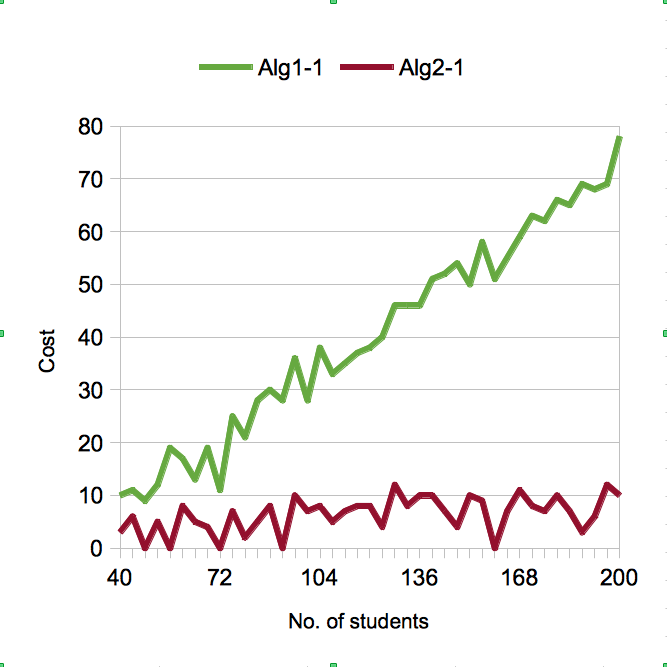
\includegraphics[width=0.45\textwidth]{report/images/rand-001.png}
		\label{fig:seq:rand}
	}
	\hfill
	\subfloat[\texttt{arc4} generator.]{
		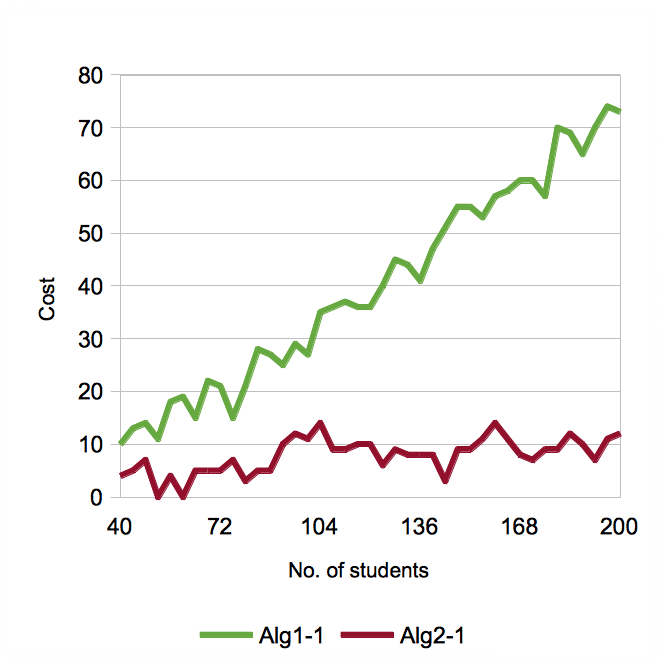
\includegraphics[width=0.45\textwidth]{report/images/arc4-01.png}
		\label{fig:seq:arc4}
	}
	\caption[Sequential solution costs]{Solution costs obtained with each approach for the sequential version with the two generators.}
	\label{fig:seq}
\end{figure*}

For the parallel version, \cref{fig:mpi:macbook} shows the results for the tests with most processes (max) and a midterm (mid) in the laptop, and \cref{fig:mpi:search} shows the results for the parallel tests using 1, 2, 4 and 8 SeARCH Group Hex nodes.

In the smaller tests, although the results still follow a similar line, \textbf{Alg1} obtained significantly better solutions in parallel, being this more noticeable in the max case. As for \textbf{Alg2}, the mid case already shows a clear improvement, and the max case obtains the perfect solution most of the times for the values chosen for $n$.

There is also a difference between the two generators. In both cases, the \texttt{rand} generator succeeded in achieving the perfect solution more times than the \texttt{arc4}. Yet, the \texttt{arc4} generator follows a very low and constant line of results, while \texttt{rand} is very irregular in the mid case, where it obtained values near the sequential results when it did not manage to find the perfect solution.

Regarding the larger tests, the improvement is considerable for both approaches. To notice that for 192 processes, the simulated annealing approach obtains the perfect solution for all the tested values of $n$.

Comparing both approaches, the parallel version greatly amplifies the distinction already present in the sequential version.

\begin{figure*}[!htp]
	\centering
	% \captionsetup[subfloat]{position=top}
	\subfloat[4 processes, \texttt{rand} generator]{
		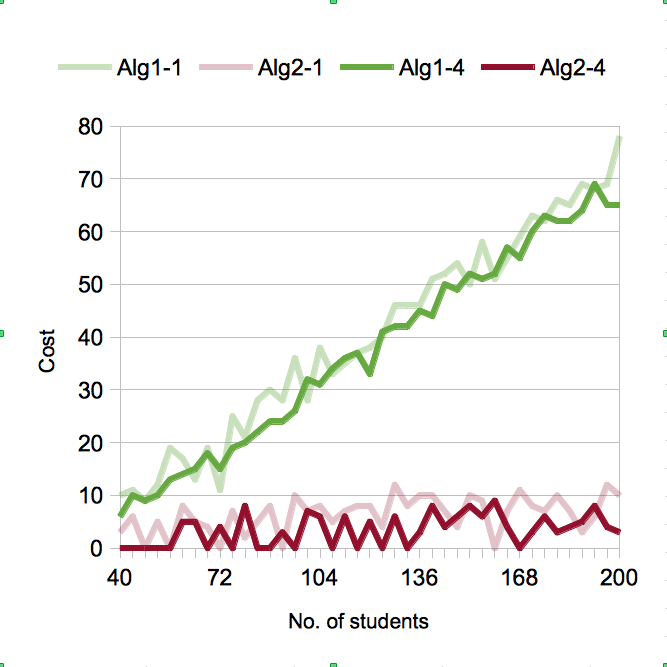
\includegraphics[width=0.45\textwidth]{report/images/rand-004.png}
		\label{fig:mpi:rand:04}
	}
	\hfill
	\subfloat[4 processes, \texttt{arc4} generator]{
		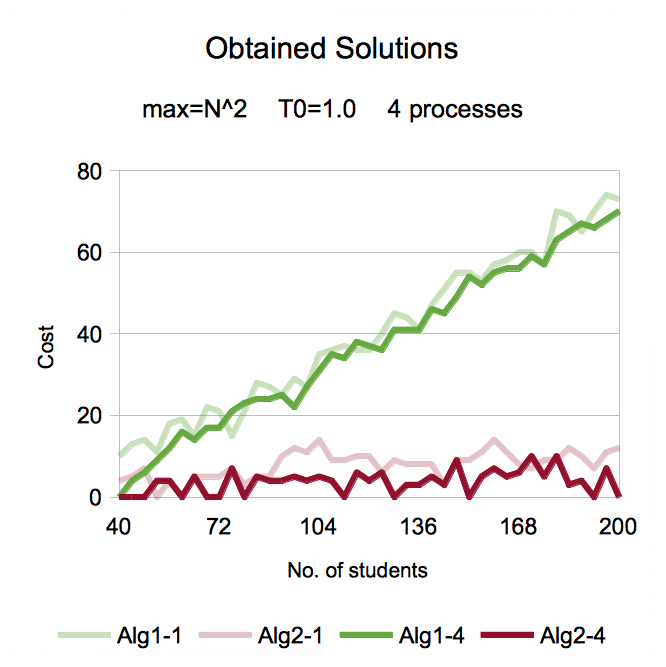
\includegraphics[width=0.45\textwidth]{report/images/arc4-04.png}
		\label{fig:mpi:arc4:04}
	}

	% \captionsetup[subfloat]{position=bottom}
	\subfloat[16 processes, \texttt{rand} generator]{
		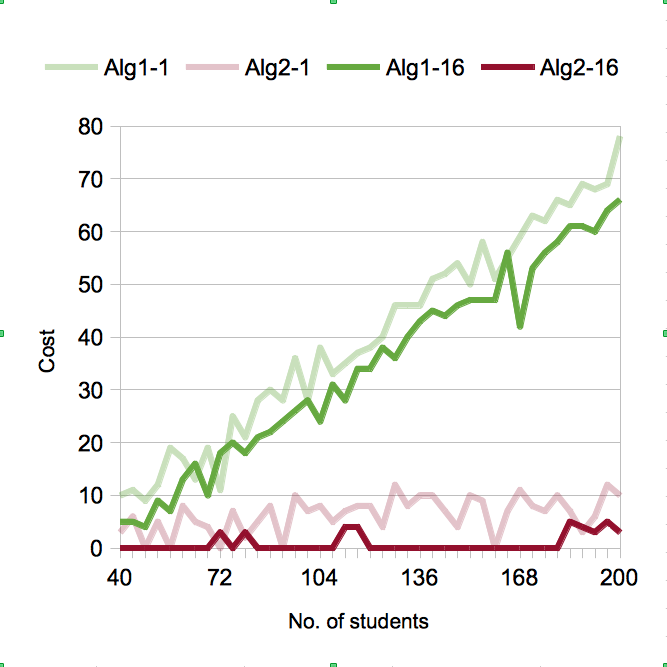
\includegraphics[width=0.45\textwidth]{report/images/rand-016.png}
		\label{fig:mpi:rand:16}
	}
	\hfill
	\subfloat[16 processes, \texttt{arc4} generator]{
		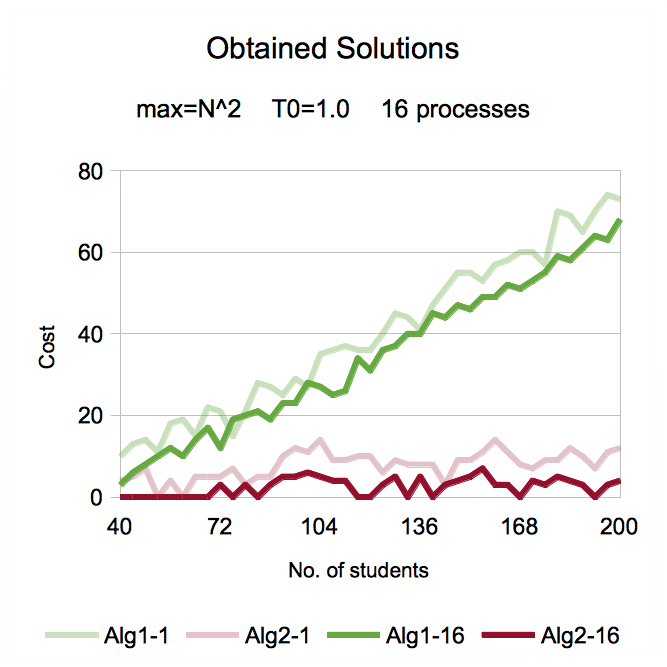
\includegraphics[width=0.45\textwidth]{report/images/arc4-16.png}
		\label{fig:mpi:arc4:16}
	}
	\caption[Parallel solution costs (up to 16)]{Solution costs obtained with each approach using the parallel version with the two generators on the MacBook Pro}
	\label{fig:mpi:macbook}
\end{figure*}

\begin{figure*}[!htp]
	\centering
	% \captionsetup[subfloat]{position=top}
	\subfloat[24 processes]{
		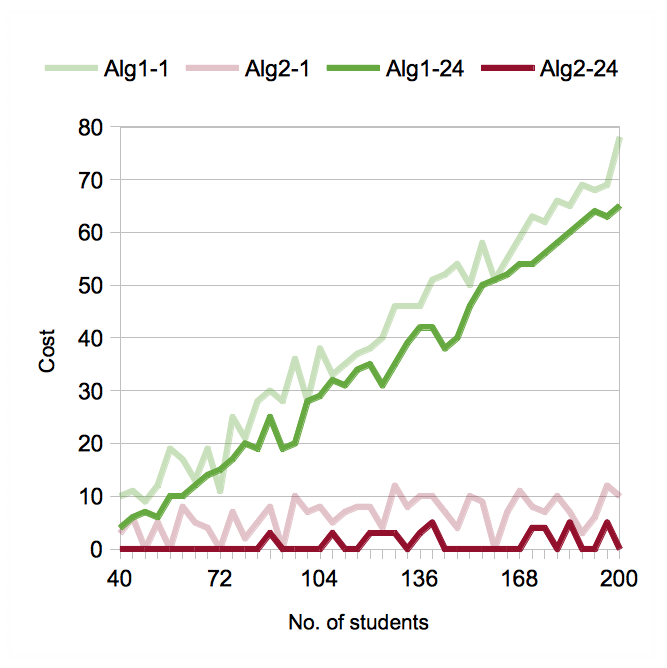
\includegraphics[width=0.45\textwidth]{report/images/rand-024.png}
		\label{fig:mpi:rand:024}
	}
	\hfill
	\subfloat[48 processes]{
		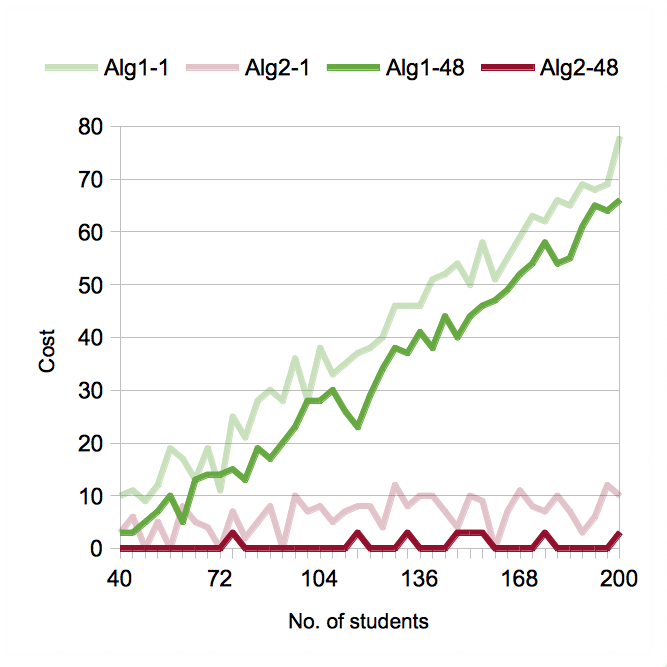
\includegraphics[width=0.45\textwidth]{report/images/rand-048.png}
		\label{fig:mpi:rand:048}
	}

	% \captionsetup[subfloat]{position=bottom}
	\subfloat[96 processes]{
		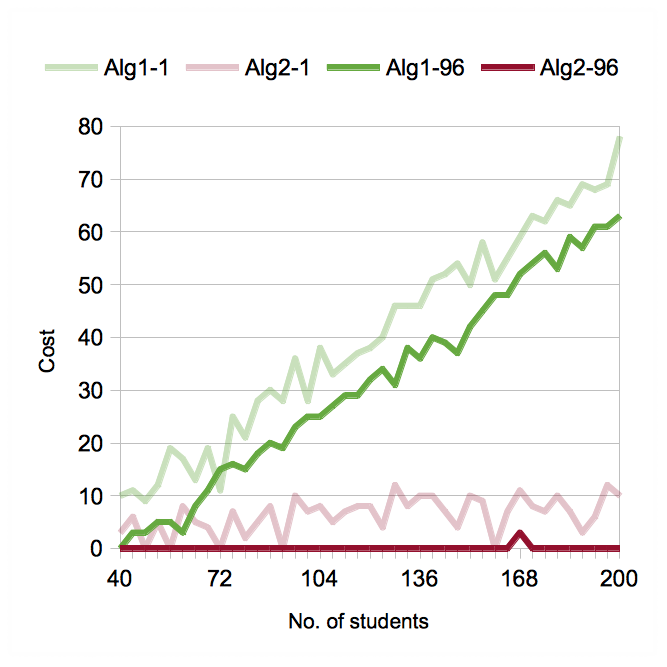
\includegraphics[width=0.45\textwidth]{report/images/rand-096.png}
		\label{fig:mpi:rand:096}
	}
	\hfill
	\subfloat[192 processes]{
		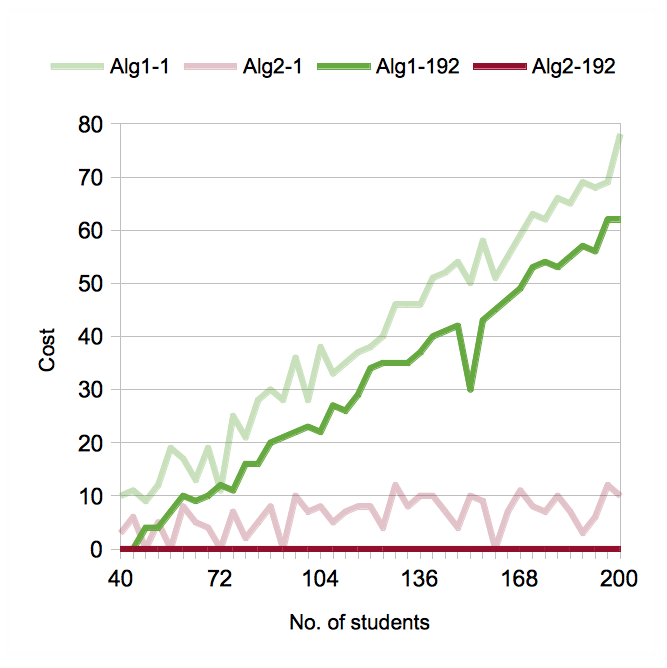
\includegraphics[width=0.45\textwidth]{report/images/rand-192.png}
		\label{fig:mpi:rand:192}
	}
	\caption[Parallel solution costs (up to 192)]{Solution costs obtained with each approach using the parallel version on SeARCH Group Hex nodes.}
	\label{fig:mpi:search}
\end{figure*}

Results regarding the influence of the initial temperature in the simulated annealing approach are shown in \cref{fig:temp:cost}. For a complete execution, the obtained costs show no significant distinction between using 1, 10 or even $10^{4}$ as the value for $T_{0}$. In \cite{Quinn2004}, the author explains that this parameter changes the method's convergence speed, and that higher values result in a slower convergence -- yet, no reference is made regarding the values of $n$ or $T_{0}$ used for the charts shown for this explanation. Although no test for larger values of $n$ completed their execution in time for this document, \cref{fig:temp:cost:limited} shows that for the first $10^{4}$ iterations, increasing the initial temperature implies obtaining worse solutions. For $T_{0}=10^{4}$, it achieves worse values than the basic approach.

\begin{figure*}[!htp]
	\centering
	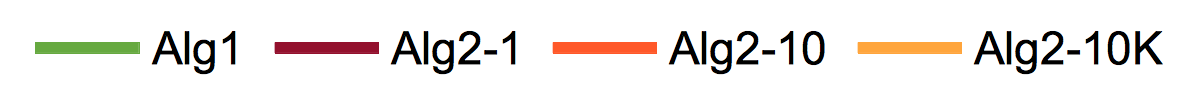
\includegraphics[width=0.7\textwidth]{report/images/temp-leg.png}

	\subfloat[Costs (complete)]{
		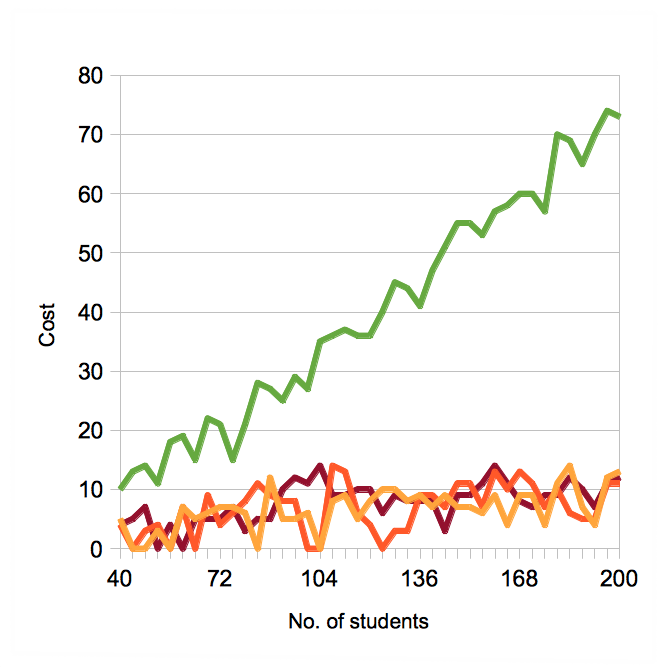
\includegraphics[width=0.45\textwidth]{report/images/temp-cost.png}
		\label{fig:temp:cost}
	}
	\hfill
	\subfloat[Costs (limited)]{
		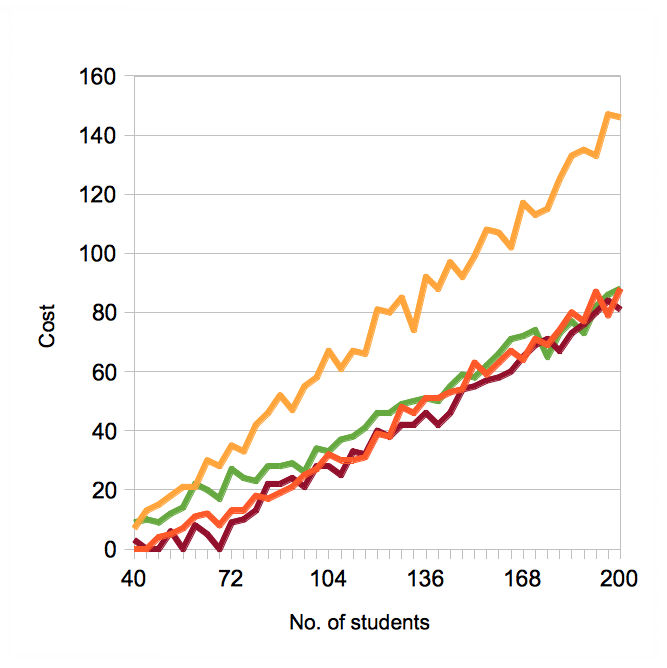
\includegraphics[width=0.45\textwidth]{report/images/temp-cost-lim.png}
		\label{fig:temp:cost:limited}
	}
	\caption[Temperature Variations]{Temperature variation results. \subref{fig:temp:cost} shows the cost of the solutions obtained with a complete execution;
	%\subref{fig:temp:iterations} shows the average number of iterations required for a complete execution; 
	\subref{fig:temp:cost:limited} shows the cost of the solution obtained after a limited number of iterations ($10^{4}$).
	}
	\label{fig:temp}
\end{figure*}
